%-------------------------------------------------------------------------------
\section{Motivation}
%-------------------------------------------------------------------------------

Developers running services on cloud provders like AWS or Google, or
containerization systems like Kubernetes, reserve the CPU and memory that
service will run on. Workloads requiring such guarantees are \textit{latency
critical} (LC). These reservations leads to a utilization problem: the load on
most applications is variable, so developers choose reservations based on the
expected peak load~\cite{borg, nu, overprovision}. \textit{Best effort} (BE)
workloads do not have reservations and their completion time is not critical.

Running BE workloads on the same resources as LCs helps solve the utilization
problem; the resource that this work focuses on is CPU. BE tasks can run on
unused CPUs opportunistically, the challenge is to enforce resource reservations
for LC services while achieving good utilization.

\begin{figure}[t]
    \centering
    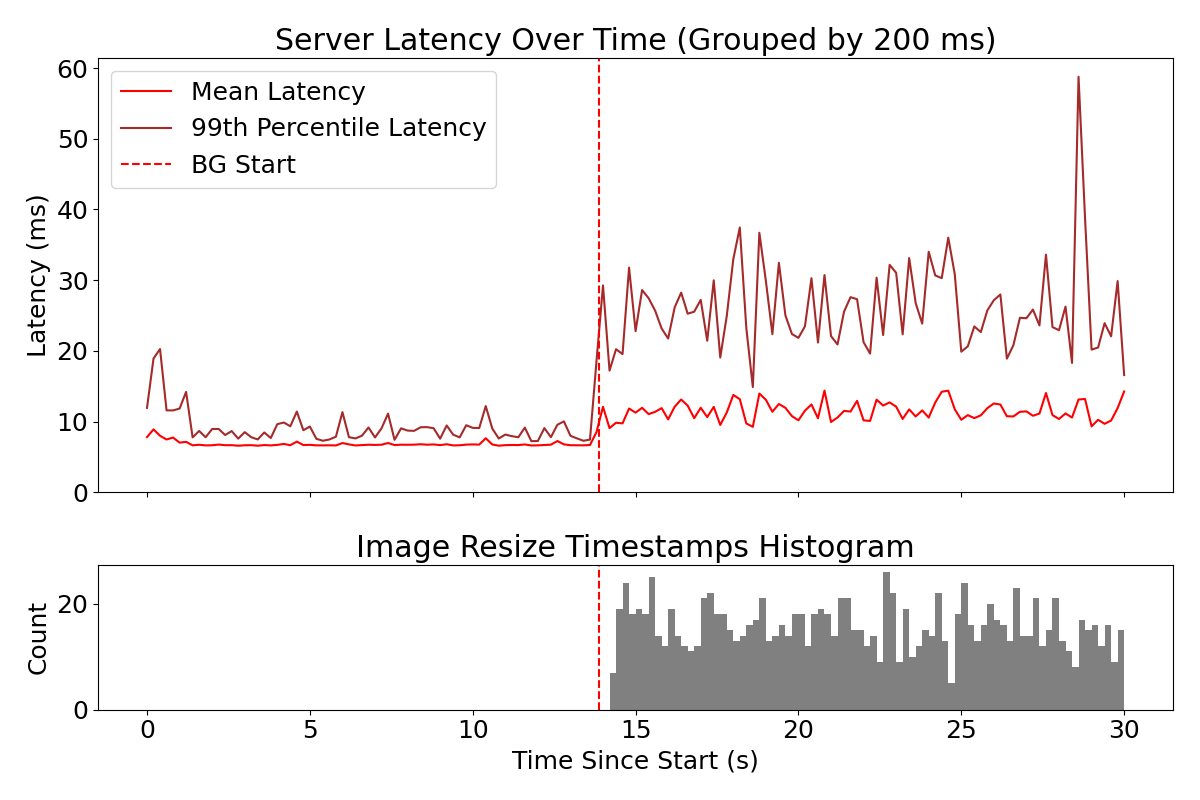
\includegraphics[width=\columnwidth]{graphs/kubernetes-unedited.png}
    \caption{In Kubernetes, running a best effort application has a latency
    impact on server that has reserved resources}\label{fig:kubernetes-unedited}
\end{figure}

Current popular scheduling systems fail to properly enforce reservations. When
running a small social web application on Kubernetes, we observe significant
impacts on its latency when starting a BE image resize job on the same cores.
$\autoref{fig:kubernetes-unedited}$ shows the end-to-end latency of an endpoint
that gets a users feed, and the throughput of the BE job. After the BE job
starts running, the mean response latency of the server jumps from $\sim$7ms to
$\sim$15ms.



